\documentclass{article}

\usepackage[preprint]{neurips_2024}
\usepackage[utf8]{inputenc}
\usepackage[T1]{fontenc}
\usepackage{hyperref}
\usepackage{url}
\usepackage{booktabs}
\usepackage{amsfonts}
\usepackage{amsmath}
\usepackage{nicefrac}
\usepackage{microtype}
\usepackage{xcolor}
\usepackage{graphicx}
\usepackage{float}
\usepackage{tikz}
\usetikzlibrary{arrows.meta,positioning,calc,fit,shapes.geometric,backgrounds}

\definecolor{paperBlue}{HTML}{2F5D9C}
\definecolor{paperCyan}{HTML}{5BB7B5}
\definecolor{paperGreen}{HTML}{66A96B}
\definecolor{paperGold}{HTML}{D8A23A}
\definecolor{paperRed}{HTML}{C75C5C}
\definecolor{paperInk}{HTML}{1F2430}
\definecolor{paperGray}{HTML}{EEF1F5}
\definecolor{paperLilac}{HTML}{B8A8E8}

\title{StreamAvatar: Real-Time-Capable Audio-Driven Portrait Animation via DyStream Optimization and Blockwise Motion Distillation}

\author{\normalfont PanChangxun \quad GuoZihan \quad LiSi}

\begin{document}
\maketitle
\begin{center}
\textbf{Project page:} \url{https://cxp-2024.github.io/StreamAvatar/}
\end{center}

\begin{abstract}
StreamAvatar is a real-time-capable audio-driven portrait animation system built by adapting and accelerating DyStream, a pretrained autoregressive flow-matching talking-head model. This report describes the resulting system. We deploy the DyStream teacher, optimize its inference path, provide an offline Gradio demo and project page, and train AROD, an Autoregressive One-step Denoising student that predicts short future motion blocks conditioned on audio, history, noisy future tokens, and reference anchors. We further study cross-attention and one-step denoising student variants, real-anchor versus synthetic-anchor conditioning, and supervised training from cached LRS3 motion latents. The optimized teacher path can approach the real-time boundary on a B20Z/B200-class GPU after warm-up, while AROD provides roughly 8$\times$ faster motion inference in a fresh 60-second verification run and has reached about 10$\times$ in the same verification setup. Our experiments show that real cached anchors give the most stable objective behavior, while mixed noise anchors sometimes improve visible motion strength and long-horizon identity consistency but do not reliably improve SyncNet metrics. The qualitative Person2 comparison is rendered as a 60-second three-way video and remains visually identity-consistent across the full long-horizon sequence. The final outcome is a StreamAvatar offline demo, a public project page, and a streaming-capable blockwise inference design, with clear empirical lessons about distilling autoregressive flow-matching portrait animation models.
\end{abstract}

%======================================================================
\section{Introduction}
%======================================================================

Audio-driven talking portrait generation synthesizes a video of a reference person or avatar speaking according to an input audio stream. It is useful for virtual meetings, low-bandwidth telepresence, privacy-preserving representation, and avatar-based communication. A practical system must satisfy three constraints at the same time: the lips should match the speech, the identity should remain stable over long clips, and inference should be fast enough for interactive use.

StreamAvatar is designed around a practical observation: a strong pretrained talking-head model already contains most of the visual prior needed for high-quality portrait animation. DyStream~\cite{dystream} provides the key components: a wav2vec-style audio front-end~\cite{wav2vec2}, an autoregressive GPT-like motion generator, a flow-matching motion sampler~\cite{flowmatching}, and a pretrained renderer. Instead of training a full portrait generator from scratch, we treat DyStream as a teacher and study how far it can be optimized, streamed, and distilled into a cheaper audio-to-motion student.

This report focuses on the implemented system. Our contribution is an engineering and modeling study of real-time-capable audio-driven portrait animation:
\begin{itemize}
    \item We deploy DyStream locally and analyze its inference bottlenecks.
    \item We build an optimized offline inference demo and analyze the requirements for extending the blockwise path to streaming playback.
    \item We train blockwise student models that predict future motion blocks directly from audio, history motion, and reference anchors.
    \item We compare real cached anchors, synthetic anchors, and mixed-anchor training, including PCA/t-SNE distribution analysis.
    \item We evaluate with SyncNet/LSE metrics~\cite{syncnet,wav2lip}, landmark-based mouth motion statistics, loss curves, qualitative videos, and speed measurements.
\end{itemize}

The main result is pragmatic. We do not claim to outperform the teacher in visual quality or to deliver a fully live video-call system. Instead, we show that the teacher path can be made practical as an offline demo and that a compact blockwise student can substantially reduce motion-generation cost, at the price of some lip-sync and motion fidelity.

%======================================================================
\section{System Overview}
%======================================================================

\begin{figure}[t]
\centering
\makebox[\textwidth][c]{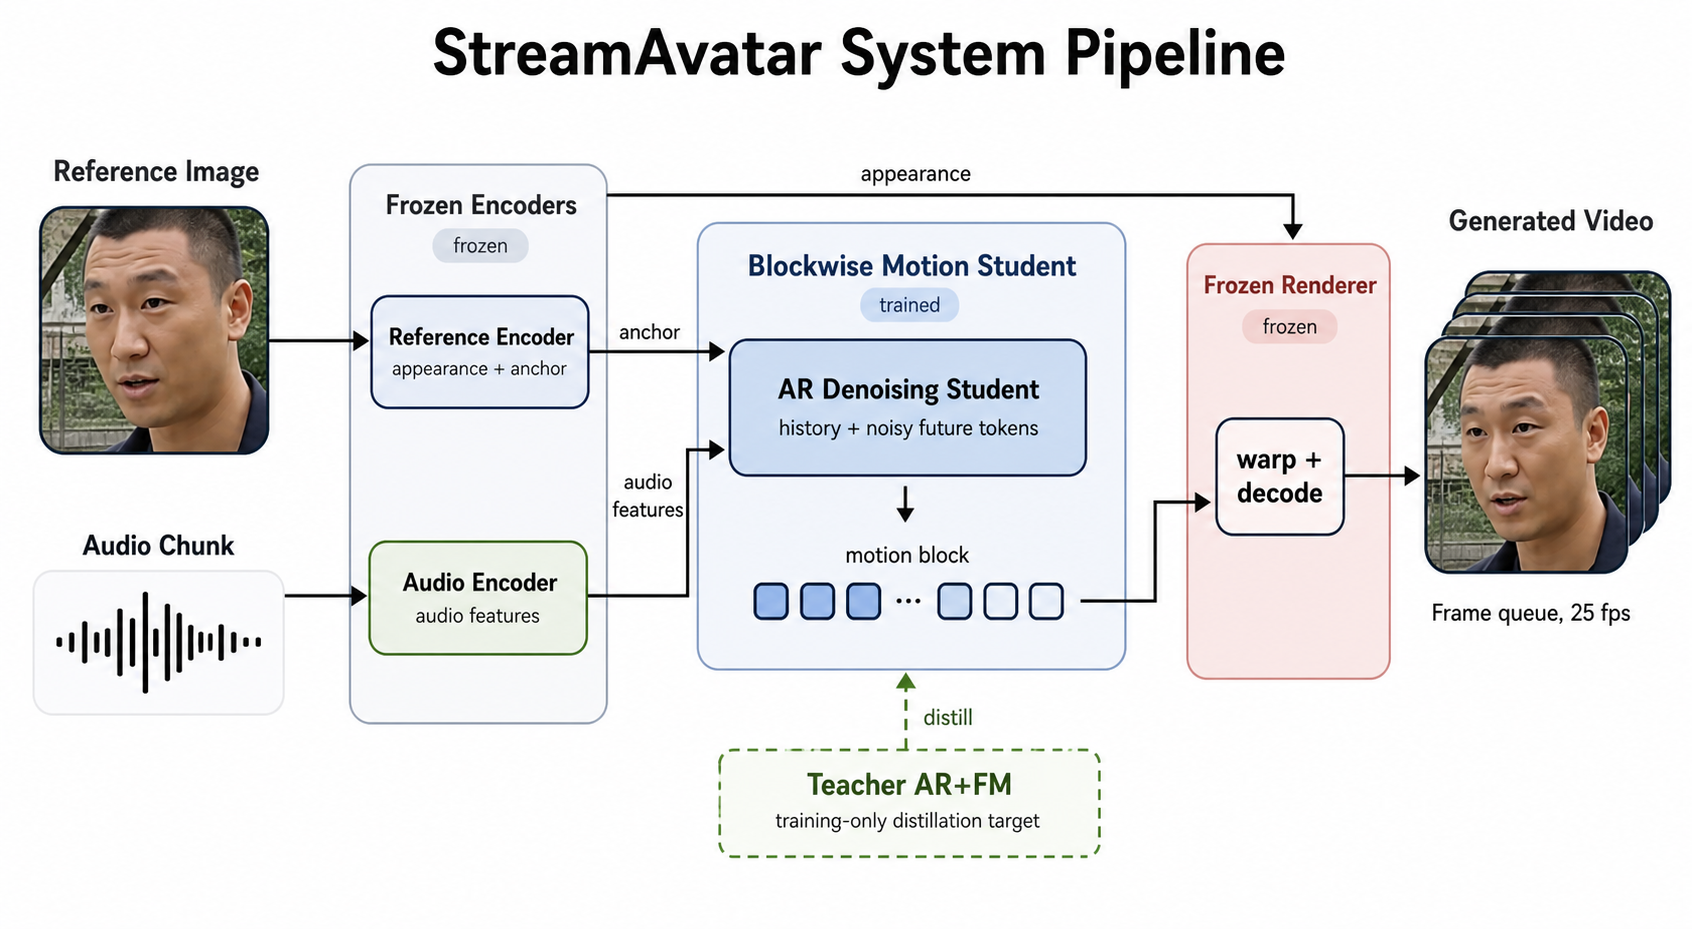
\includegraphics[width=1.0\textwidth]{figures/system_pipeline_imagegen.png}}
\caption{Final StreamAvatar system. The original DyStream teacher is preserved as the quality reference. Our student path bypasses the expensive AR+FM teacher rollout by predicting short motion blocks directly from audio, history, and anchors.}
\label{fig:overview}
\end{figure}

\iffalse
\begin{figure}[t]
\centering
\resizebox{\textwidth}{!}{%
\begin{tikzpicture}[x=1cm,y=1cm,>=Latex,font=\small,
  stage/.style={draw=paperInk!80,fill=#1!10,rounded corners=2mm,minimum width=2.15cm,minimum height=0.88cm,align=center,inner sep=4pt,line width=0.95pt},
  latent/.style={draw=paperInk!75,fill=#1!30,rounded corners=1mm,minimum width=0.34cm,minimum height=0.34cm,line width=0.8pt},
  arrow/.style={->,draw=paperInk,line width=1.0pt},
  label/.style={font=\scriptsize,text=paperInk}
]
  \node[font=\bfseries\Large,text=paperInk] at (8.0,5.20) {System pipeline};

  \node[font=\bfseries\large,text=paperInk] at (1.50,4.55) {Reference Image};
  \node[inner sep=0pt,draw=paperInk!55,line width=0.9pt,rounded corners=2mm] (refimg) at (1.50,3.25)
    {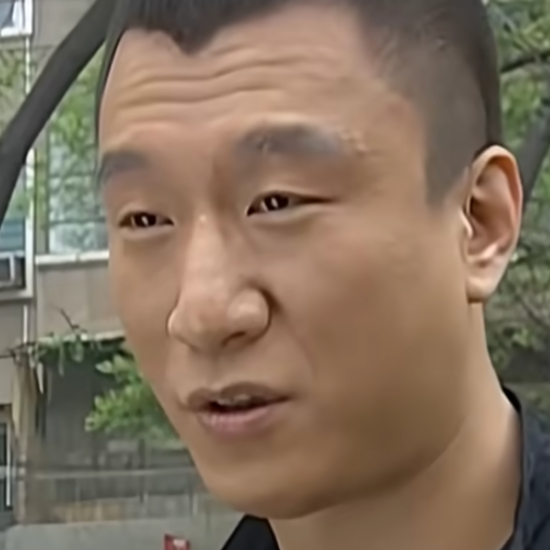
\includegraphics[width=2.05cm,height=2.05cm]{figures/reference_person2.png}};

  \draw[rounded corners=2mm,fill=paperGray,draw=none] (0.32,0.45) rectangle (2.68,1.78);
  \node[label] at (1.50,1.48) {audio stream};
  \draw[draw=paperInk,line width=1.0pt] (0.62,1.06) -- (0.80,1.06) -- (0.90,1.26) -- (1.02,0.84) --
    (1.16,1.42) -- (1.30,0.75) -- (1.45,1.33) -- (1.58,0.90) -- (1.72,1.18) --
    (1.88,1.00) -- (2.05,1.10) -- (2.22,1.06);

  \node[stage=paperCyan,minimum width=0.95cm,minimum height=2.70cm] (enc) at (4.0,3.05) {\rotatebox{90}{Frozen encoder}};
  \node[latent=paperCyan] (app) at (5.25,3.85) {};
  \node[font=\itshape\scriptsize,text=paperInk] at (5.95,4.18) {appearance};
  \node[latent=paperCyan] (m0) at (5.25,2.35) {};
  \node[font=\itshape\scriptsize,text=paperInk] at (5.78,2.02) {anchor $m^0$};

  \draw[arrow] (refimg.east) -- (enc.west);
  \draw[arrow] (enc.east) -- (app.west);
  \draw[arrow] (enc.east) -- (m0.west);

  \draw[rounded corners=4mm,fill=paperGray,draw=none] (5.75,0.78) rectangle (11.05,3.35);
  \node[font=\bfseries,text=paperInk] at (8.40,3.05) {Audio-to-Motion Generator};
  \node[stage=paperGold,minimum width=3.10cm,minimum height=0.82cm] (student) at (8.40,1.30)
    {blockwise student\\{\scriptsize audio + history + anchor}};
  \foreach \i/\c in {0/paperCyan,1/paperBlue,2/paperCyan,3/paperBlue,4/paperCyan} {
    \node[latent=\c] (tok\i) at (7.10+\i*0.65,2.28) {};
  }
  \node[font=\scriptsize,text=paperInk] at (8.40,2.72) {$m^{1:N}$ motion latents};
  \draw[arrow] (2.68,1.12) -- node[below,label] {$a^{1:N}$} (student.west);
  \draw[arrow] (m0.south) |- (student.west);
  \draw[arrow] (student.north) -- (tok2.south);

  \node[stage=paperGreen,minimum width=2.35cm] (teacher) at (8.40,4.15) {teacher AR+FM\\{\scriptsize distillation target}};
  \draw[arrow,dashed,draw=paperGreen] (2.68,1.38) .. controls (4.4,4.7) and (6.4,4.65) .. (teacher.west);
  \draw[arrow,dashed,draw=paperGreen] (teacher.south) -- node[right,label] {pseudo motion} (tok2.north);

  \node[draw=paperInk!85,fill=white,circle,minimum size=0.52cm,line width=0.95pt] (warp) at (11.72,3.12) {$w$};
  \node[font=\itshape\scriptsize,text=paperInk] at (11.72,3.62) {warping};
  \node[stage=paperRed,minimum width=0.95cm,minimum height=2.70cm] (dec) at (12.85,3.05) {\rotatebox{90}{Renderer}};
  \node[font=\bfseries\large,text=paperInk] at (15.10,4.55) {Generated Video};
  \node[inner sep=0pt,draw=paperInk!30,line width=0.6pt,rounded corners=2mm] at (14.82,3.10)
    {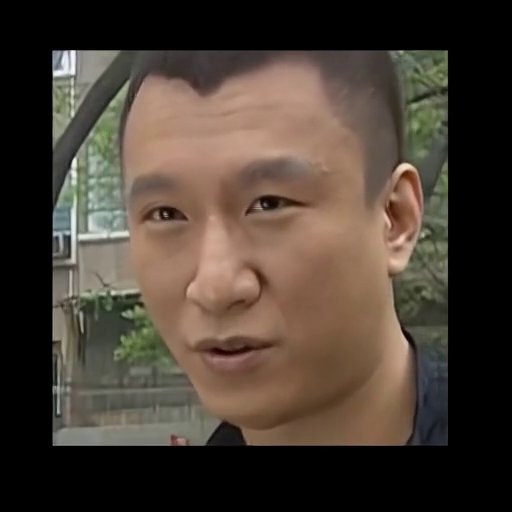
\includegraphics[width=1.88cm,height=1.88cm]{figures/generated_person2_frame.png}};
  \node[inner sep=0pt,draw=paperInk!45,line width=0.7pt,rounded corners=2mm] at (15.06,3.25)
    {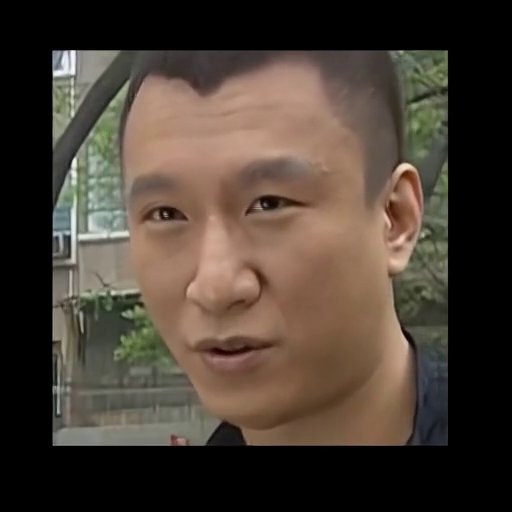
\includegraphics[width=1.88cm,height=1.88cm]{figures/generated_person2_frame.png}};
  \node[inner sep=0pt,draw=paperInk!65,line width=0.9pt,rounded corners=2mm] (gen) at (15.30,3.40)
    {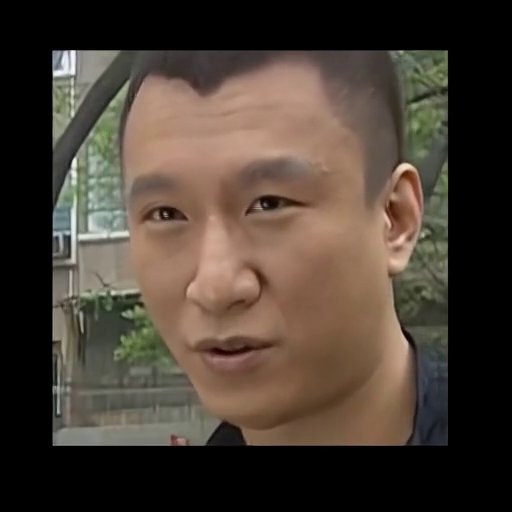
\includegraphics[width=1.88cm,height=1.88cm]{figures/generated_person2_frame.png}};
  \node[label] at (15.30,1.96) {frame queue, 25 fps};

  \draw[arrow] (app.east) -- node[above,label] {$v_{\mathrm{app}}$} (warp.west);
  \draw[arrow] (tok4.east) -| (warp.south);
  \draw[arrow] (warp.east) -- (dec.west);
  \draw[arrow] (dec.east) -- (gen.west);
\end{tikzpicture}
}
\caption{Final StreamAvatar system. The original DyStream teacher is preserved as the quality reference. Our student path bypasses the expensive AR+FM teacher rollout by predicting short motion blocks directly from audio, history, and anchors.}
\label{fig:overview}
\end{figure}
\fi

DyStream is naturally modular. The model does not generate pixels directly from audio. Instead, audio is encoded into temporal features, an autoregressive motion model predicts a latent motion trajectory, flow matching refines or samples the motion latent, and a pretrained renderer turns the motion into video frames. This is important for real-time work because the expensive pixel-level identity and appearance prior can remain frozen.

In our optimized runtime, the teacher path is used in two ways. First, it is the baseline used for qualitative comparison. Second, it provides pseudo-targets for distillation: for a fixed audio chunk and reference anchor, the teacher produces a motion trajectory, and the student learns to produce a similar trajectory with fewer sequential operations.

%======================================================================
\section{Method}
%======================================================================

\subsection{Optimized DyStream Inference}

We first made the DyStream inference path usable as a local application. The important optimizations were not all model-level. Model loading is moved out of the hot path, the reference image is preprocessed once, rendering is batched, and the web app reports stage-level timing. The best practical setting used a small motion chunk size and batched rendering. In our profiling, the original teacher path remains close to the real-time boundary rather than being an order of magnitude faster: a 60-second baseline run was dominated by motion generation and rendering, while warmed-up short-clip tests were around real-time. The large speedup reported later therefore refers to the distilled student motion rollout, not to the full DyStream teacher pipeline.

The current application interface is an offline Gradio demo: a user provides a reference image and an audio file, the backend predicts the full motion sequence, and the renderer writes the output video. A live version would require an additional frame queue, microphone noise handling, browser-side scheduling, and rolling backend state. We treat these as streaming-system requirements rather than claims about the current delivered app.

\subsection{Blockwise Student Distillation}

The teacher uses an autoregressive structure. A GPT-like model conditions on previous motion and audio, then the flow-matching module generates motion latents. This is high quality but sequential. We call our final student \textbf{AROD}, short for \textit{Autoregressive One-step Denoising}. AROD should be understood as a blockwise autoregressive denoising model, not as the teacher's two-stage AR+FM pipeline. For each block, it receives rolling motion history, audio features, a reference anchor, noisy future tokens, and a timestep, then directly predicts a clean future motion block:
\begin{equation}
    \hat{\mathbf{M}}_{t:t+B-1}
    =
    f_\theta(
      \mathbf{A}_{t:t+B-1},
      \mathbf{M}_{t-H:t-1},
      \mathbf{r},
      \mathbf{Z}_{t:t+B-1},
      \tau
    ),
\end{equation}
where $B=2$ in our conservative final student, $H$ is the history length, $\mathbf{A}$ denotes audio features, $\mathbf{r}$ is the reference anchor, $\mathbf{Z}$ denotes noisy future-token input, and $\tau$ is the sampled timestep. During rollout, the predicted block is appended to history and used by the next block.

\begin{figure}[t]
\centering
\makebox[\textwidth][c]{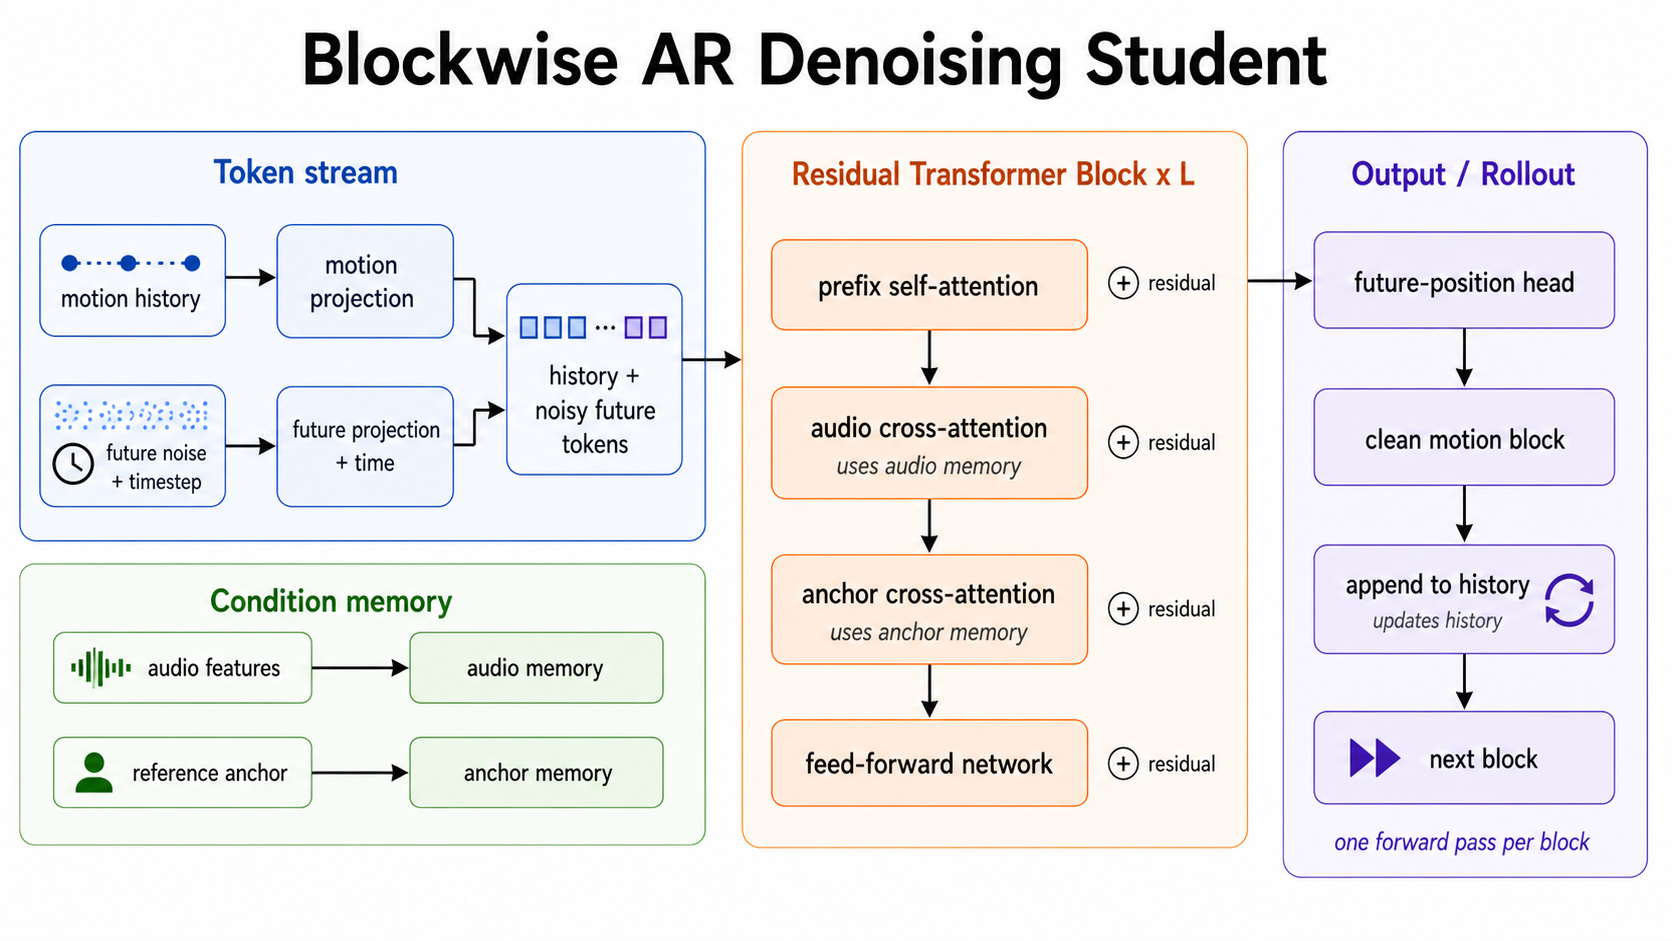
\includegraphics[width=1.0\textwidth]{figures/student_arch_imagegen.png}}
\caption{Blockwise AR denoising student. Noisy future tokens are part of the Transformer input, not a separate ODE sampler. The model performs one forward pass per block, outputs the clean future motion block, appends it to history, and then predicts the next block.}
\label{fig:student}
\end{figure}

\iffalse
\begin{figure}[t]
\centering
\resizebox{\textwidth}{!}{%
\begin{tikzpicture}[x=1cm,y=1cm,>=Latex,font=\small,
  token/.style={draw=paperInk!70,fill=#1!34,rounded corners=1mm,minimum width=0.46cm,minimum height=0.46cm,line width=0.85pt},
  block/.style={draw=paperInk!80,fill=#1!15,rounded corners=1.6mm,minimum width=3.45cm,minimum height=0.58cm,align=center,line width=0.9pt},
  box/.style={draw=paperInk!80,fill=#1!10,rounded corners=2mm,minimum width=2.30cm,minimum height=0.72cm,align=center,line width=0.9pt},
  arrow/.style={->,draw=paperInk,line width=0.95pt},
  lab/.style={font=\scriptsize,text=paperInk}
]
  \node[font=\bfseries\Large,text=paperInk] at (7.60,6.10) {Blockwise Audio-to-Motion Student};

  \draw[rounded corners=4mm,fill=paperBlue!10,draw=none] (0.35,0.55) rectangle (10.85,5.55);
  \draw[rounded corners=4mm,fill=paperRed!8,draw=none] (11.12,0.55) rectangle (15.20,5.55);

  \node[font=\bfseries,text=paperInk] at (1.62,4.92) {Reference};
  \node[inner sep=0pt,draw=paperInk!45,line width=0.8pt,rounded corners=2mm] (ref2) at (1.62,3.95)
    {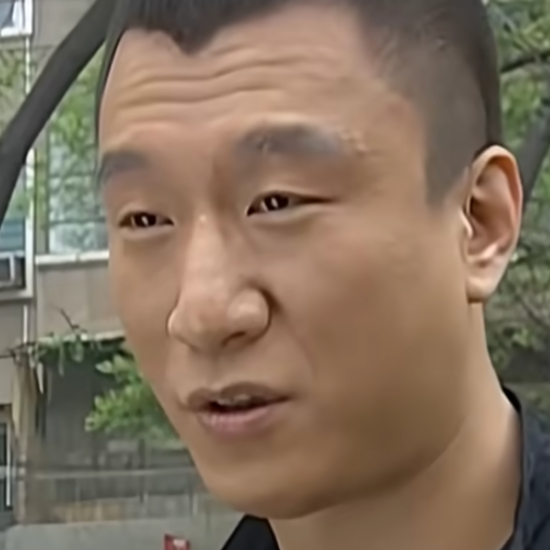
\includegraphics[width=1.15cm,height=1.15cm]{figures/reference_person2.png}};
  \node[box=paperCyan,minimum width=0.72cm,minimum height=1.34cm] (enc2) at (3.02,3.95) {\rotatebox{90}{Encoder}};
  \node[token=paperCyan] (anc) at (4.18,3.95) {};
  \node[lab] at (4.20,3.52) {anchor};
  \draw[arrow] (ref2.east) -- (enc2.west);
  \draw[arrow] (enc2.east) -- (anc.west);

  \node[font=\itshape\large,text=paperInk] at (5.72,5.00) {$m^{t-H:t-1}$};
  \foreach \i/\c in {0/paperBlue,1/paperCyan,2/paperCyan,3/paperBlue,4/paperCyan,5/paperCyan,6/paperBlue} {
    \node[token=\c] (mh\i) at (4.72+\i*0.62,4.45) {};
  }
  \node[token=paperGold,dashed] (future) at (9.28,4.45) {};
  \node[lab] at (9.28,4.03) {future};

  \draw[rounded corners=2mm,fill=white,draw=paperInk!35,line width=0.7pt] (0.88,1.02) rectangle (3.85,2.28);
  \node[lab] at (1.62,2.02) {speaker};
  \node[lab] at (1.62,1.30) {listener};
  \draw[draw=paperInk,line width=0.9pt] (2.12,2.02) -- (2.25,2.02) -- (2.34,2.18) -- (2.45,1.83) --
    (2.56,2.24) -- (2.68,1.82) -- (2.80,2.08) -- (2.94,1.96) -- (3.10,2.02);
  \draw[draw=paperInk,line width=0.9pt] (2.12,1.30) -- (2.25,1.30) -- (2.34,1.47) -- (2.45,1.10) --
    (2.56,1.55) -- (2.68,1.08) -- (2.80,1.37) -- (2.94,1.24) -- (3.10,1.30);
  \node[box=paperGray,minimum width=2.05cm] (spk) at (4.72,2.02) {speaker encoder};
  \node[box=paperGray,minimum width=2.05cm] (lst) at (4.72,1.22) {listener encoder};
  \node[draw=paperInk,circle,fill=white,minimum size=0.46cm] (plus) at (6.12,1.62) {$+$};
  \draw[arrow] (3.85,2.02) -- (spk.west);
  \draw[arrow] (3.85,1.22) -- (lst.west);
  \draw[arrow] (spk.east) -- (plus.north west);
  \draw[arrow] (lst.east) -- (plus.south west);

  \node[block=paperCyan,minimum width=4.0cm] (b1) at (8.08,3.30) {causal self-attention};
  \node[block=paperCyan,minimum width=4.0cm] (b2) at (8.08,2.52) {audio cross-attention};
  \node[block=paperCyan,minimum width=4.0cm] (b3) at (8.08,1.74) {anchor cross-attention};
  \node[block=paperCyan,minimum width=4.0cm] (b4) at (8.08,0.96) {MLP residual};
  \node[font=\large,text=paperInk] at (10.38,2.12) {$\times L_A$};

  \draw[arrow] (mh3.south) -- (b1.north);
  \draw[arrow] (plus.east) -- (b2.west);
  \draw[arrow] (anc.east) |- (b3.west);
  \draw[arrow] (b1.south) -- (b2.north);
  \draw[arrow] (b2.south) -- (b3.north);
  \draw[arrow] (b3.south) -- (b4.north);

  \node[font=\bfseries,text=paperInk] at (13.15,5.02) {FM-style head};
  \node[token=paperGray] (noisy) at (13.05,1.05) {};
  \node[lab] at (12.20,1.05) {noisy motion};
  \node[box=paperCyan,minimum width=0.62cm] (time) at (14.42,1.05) {$t$};
  \node[block=paperGold,minimum width=2.45cm] (f1) at (13.05,2.00) {AdaLN};
  \node[block=paperGold,minimum width=2.45cm] (f2) at (13.05,2.75) {MLP};
  \node[block=paperGold,minimum width=2.45cm] (f3) at (13.05,3.50) {AdaLN};
  \node[block=paperGold,minimum width=2.45cm] (f4) at (13.05,4.25) {MLP};
  \node[token=paperCyan,dashed] (clean) at (13.05,4.88) {};
  \node[lab] at (12.05,4.88) {clean motion};
  \node[font=\large,text=paperInk] at (14.72,3.05) {$\times L_F$};

  \draw[arrow] (b4.east) -- node[above,lab] {$c^t$} (f2.west);
  \draw[arrow] (noisy.north) -- (f1.south);
  \draw[arrow] (f1.north) -- (f2.south);
  \draw[arrow] (f2.north) -- (f3.south);
  \draw[arrow] (f3.north) -- (f4.south);
  \draw[arrow] (f4.north) -- (clean.south);
  \draw[arrow] (time.west) -- (f1.east);
  \draw[arrow] (time.west) |- (f3.east);
  \draw[arrow] (clean.west) -- node[above,lab] {$m^{t:t+B-1}$} (9.90,4.88) |- (future.north);
\end{tikzpicture}
}
\caption{Blockwise AR denoising student. Noisy future tokens are part of the Transformer input, and the model predicts a clean short motion block with one forward pass.}
\label{fig:student}
\end{figure}
\fi

We explored several student architectures. The most useful version is AROD's blockwise cross-attention denoising student. History tokens and noisy future tokens are processed in one Transformer sequence. Audio and anchor features are injected through cross-attention. The retained ``FM-like'' part is only the noise/timestep interface: during training we create a noisy version of the target future block, and during inference we feed Gaussian future noise at the first scheduler timestep. The student does not run an ODE solver and does not predict a velocity field; it directly predicts clean motion in one forward pass per block.

\subsection{Training Objectives}

The student is trained by rollout. For a training clip, we run the student block by block. Each predicted block is appended to the history for the following block. Gradients are accumulated through the rollout inside one forward/backward step, with optional detachment between blocks for stability. The main loss compares the predicted motion block against either teacher motion or cached real motion:
\begin{equation}
    \mathcal{L}_{\text{motion}} =
    \| \hat{\mathbf{M}} - \mathbf{M}^\star \|_2^2.
\end{equation}
We additionally use velocity, acceleration, and boundary losses:
\begin{equation}
    \mathcal{L}
    =
    \mathcal{L}_{\text{motion}}
    + \lambda_v \mathcal{L}_{\text{velocity}}
    + \lambda_a \mathcal{L}_{\text{acceleration}}
    + \lambda_b \mathcal{L}_{\text{boundary}}.
\end{equation}
The velocity and acceleration losses discourage slow-motion collapse and unnatural jitter. The boundary loss makes adjacent predicted blocks connect smoothly.

\subsection{Anchor Conditioning}

The reference anchor is a 512-dimensional motion/identity-style latent extracted from the reference image or cached training video. We tested three anchor regimes:
\begin{itemize}
    \item \textbf{Real anchor}: use cached real anchors from LRS3 motion latents.
    \item \textbf{Noise anchor}: use synthetic Gaussian or sphere noise anchors.
    \item \textbf{Mixed anchor}: use real anchors for half the batch and synthetic anchors for the other half.
\end{itemize}
The mixed-sphere variant samples
\begin{equation}
    \mathbf{r}_{\text{noise}} =
    \bar{\mathbf{r}}_{\text{real}}
    +
    R \cdot
    \frac{\epsilon}{\|\epsilon\|_2},
    \quad \epsilon \sim \mathcal{N}(0,I),
\end{equation}
with $R=6$. This was intended to cover the real-anchor distribution. However, later PCA analysis showed that high-dimensional sphere sampling does not expand along the true principal directions of real anchors. It is therefore better interpreted as a regularizer than as faithful distribution coverage.

%======================================================================
\section{Experiments}
%======================================================================

\subsection{Data and Setup}

We use LRS3~\cite{lrs3} video/audio clips. Two kinds of targets are used. Teacher-distillation targets are generated online by the DyStream teacher. Cached-real targets are generated by preprocessing LRS3 videos into audio waveforms and 512-dimensional motion-latent sequences. For the largest student runs, we used a 60k pretrain-cache manifest with a held-out validation set. Most clips are sampled as 3-second training segments to keep training efficient and compatible with blockwise rollout.

The renderer and teacher components remain frozen. The student is trained with batch size 64 in the main cache/anchor experiments. Validation is run periodically and logged to JSONL. All reported qualitative comparisons use the same audio/reference inputs for teacher and student.

\subsection{Metrics}

We report the following metrics:
\begin{itemize}
    \item \textbf{LSE-D}: SyncNet audio-video distance; lower is better.
    \item \textbf{LSE-C}: SyncNet confidence; higher is better.
    \item \textbf{Mouth-audio correlation}: correlation between landmark mouth opening and audio energy.
    \item \textbf{Mouth velocity}: average landmark mouth-opening velocity, used as a rough motion-strength indicator.
    \item \textbf{Motion MSE/L1}: latent distance between student and teacher motion.
    \item \textbf{Velocity ratio}: student/teacher motion velocity magnitude. Values closer to one indicate less under-motion.
    \item \textbf{Speedup}: measured student motion rollout speed relative to the teacher rollout in verification.
\end{itemize}

\subsection{Main Quantitative Results}

\begin{table}[t]
\centering
\scriptsize
\setlength{\tabcolsep}{3.2pt}
\resizebox{\textwidth}{!}{%
\begin{tabular}{@{}lrrrrrr@{}}
\toprule
\textbf{Model} & \textbf{LSE-D} $\downarrow$ & \textbf{LSE-C} $\uparrow$ & \textbf{Mouth corr.} $\uparrow$ & \textbf{Mouth vel.} & \textbf{Motion MSE} $\downarrow$ & \textbf{Vel. ratio} \\
\midrule
Teacher & \textbf{7.679} & \textbf{4.987} & \textbf{0.305} & \textbf{0.0346} & -- & -- \\
Real-anchor student & 8.853 & \textbf{4.054} & 0.225 & 0.0276 & \textbf{0.0257} & 0.678 \\
Noise+real student & \textbf{8.721} & 4.036 & \textbf{0.238} & \textbf{0.0305} & 0.0277 & \textbf{0.774} \\
\bottomrule
\end{tabular}
}
\caption{Person1 60-second comparison. Teacher is best overall. Mixed anchors increase visible motion strength and improve velocity ratio, while real anchors better match teacher latents.}
\label{tab:person1}
\end{table}

\begin{table}[t]
\centering
\scriptsize
\setlength{\tabcolsep}{2.8pt}
\resizebox{\textwidth}{!}{%
\begin{tabular}{@{}lrrrrrrr@{}}
\toprule
\textbf{Model} & \textbf{LSE-D} $\downarrow$ & \textbf{LSE-C} $\uparrow$ & \textbf{Mouth corr.} $\uparrow$ & \textbf{Mouth vel.} & \textbf{Motion MSE} $\downarrow$ & \textbf{Vel. ratio} & \textbf{Speedup} \\
\midrule
Teacher & \textbf{7.080} & \textbf{6.235} & 0.051 & 0.0326 & -- & -- & -- \\
Real-anchor student & \textbf{8.309} & \textbf{4.027} & 0.0328 & 0.0336 & \textbf{0.0305} & 0.760 & \textbf{8.47$\times$} \\
Noise+real student & 8.429 & 3.280 & \textbf{0.0789} & \textbf{0.0359} & 0.0384 & \textbf{0.832} & 7.71$\times$ \\
\bottomrule
\end{tabular}
}
\caption{Person2 60-second comparison. Real anchors are better on SyncNet and latent matching; mixed anchors produce stronger mouth motion. The corresponding three-way rendered video remains visually identity-consistent over the full long-horizon clip.}
\label{tab:person2}
\end{table}

The teacher remains the quality reference. Between students, the result is mixed. Real-anchor training gives more conservative and stable teacher-latent imitation. Noise+real mixed anchors can improve visible mouth motion strength and velocity magnitude, but the SyncNet improvement is not consistent across reference images. Qualitatively, the 60-second Person2 three-way comparison keeps the same facial identity and appearance traits across the long clip, which is important for practical avatar use: the student does not collapse into a different identity after extended autoregressive rollout.

\subsection{Training Curves and Anchor Analysis}

\begin{figure}[t]
\centering
\begin{minipage}{0.48\textwidth}
  \centering
  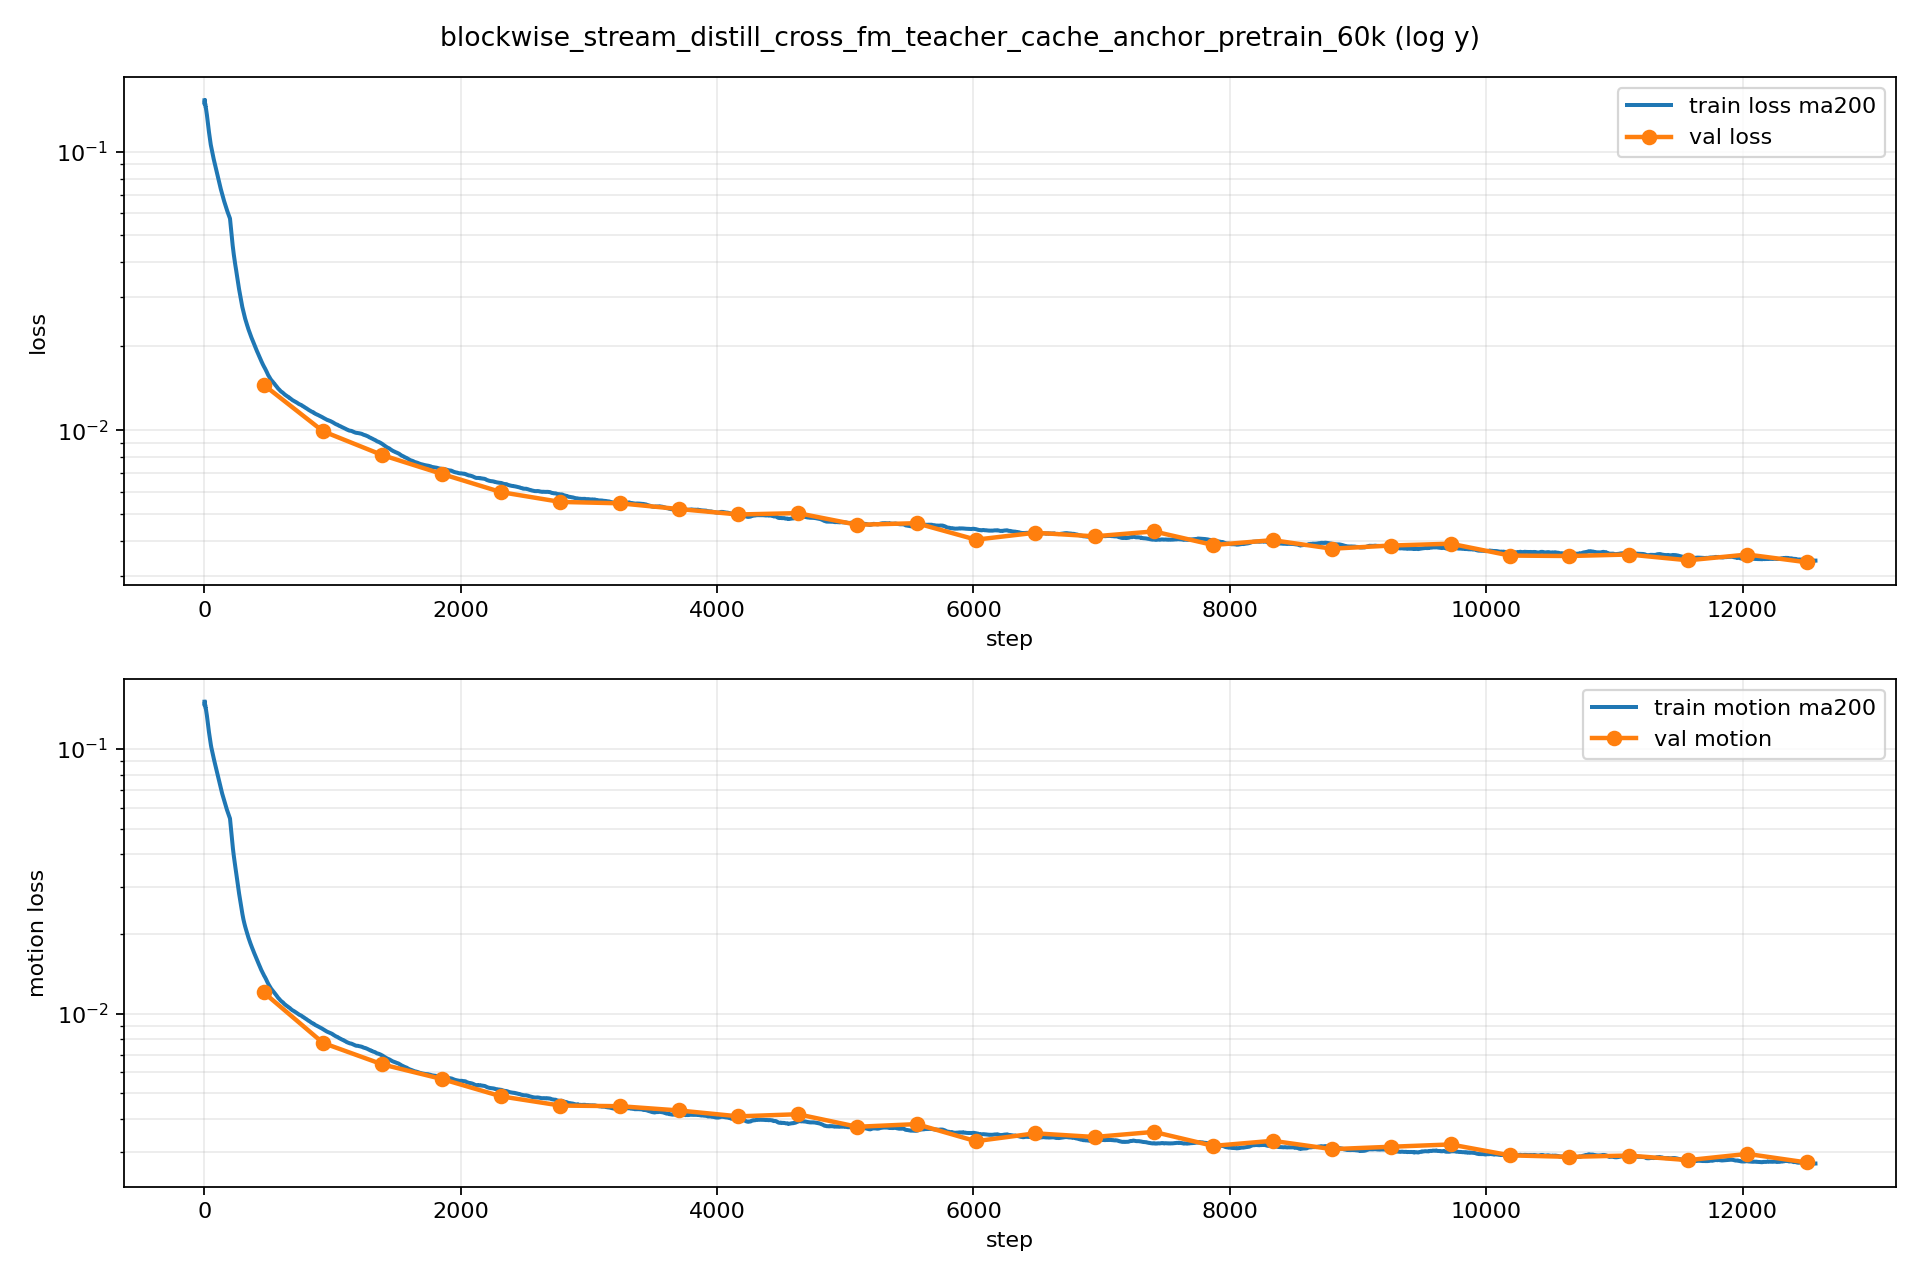
\includegraphics[width=\linewidth]{figures/loss_real_anchor_log.png}
  {\small Real-anchor student}
\end{minipage}
\hfill
\begin{minipage}{0.48\textwidth}
  \centering
  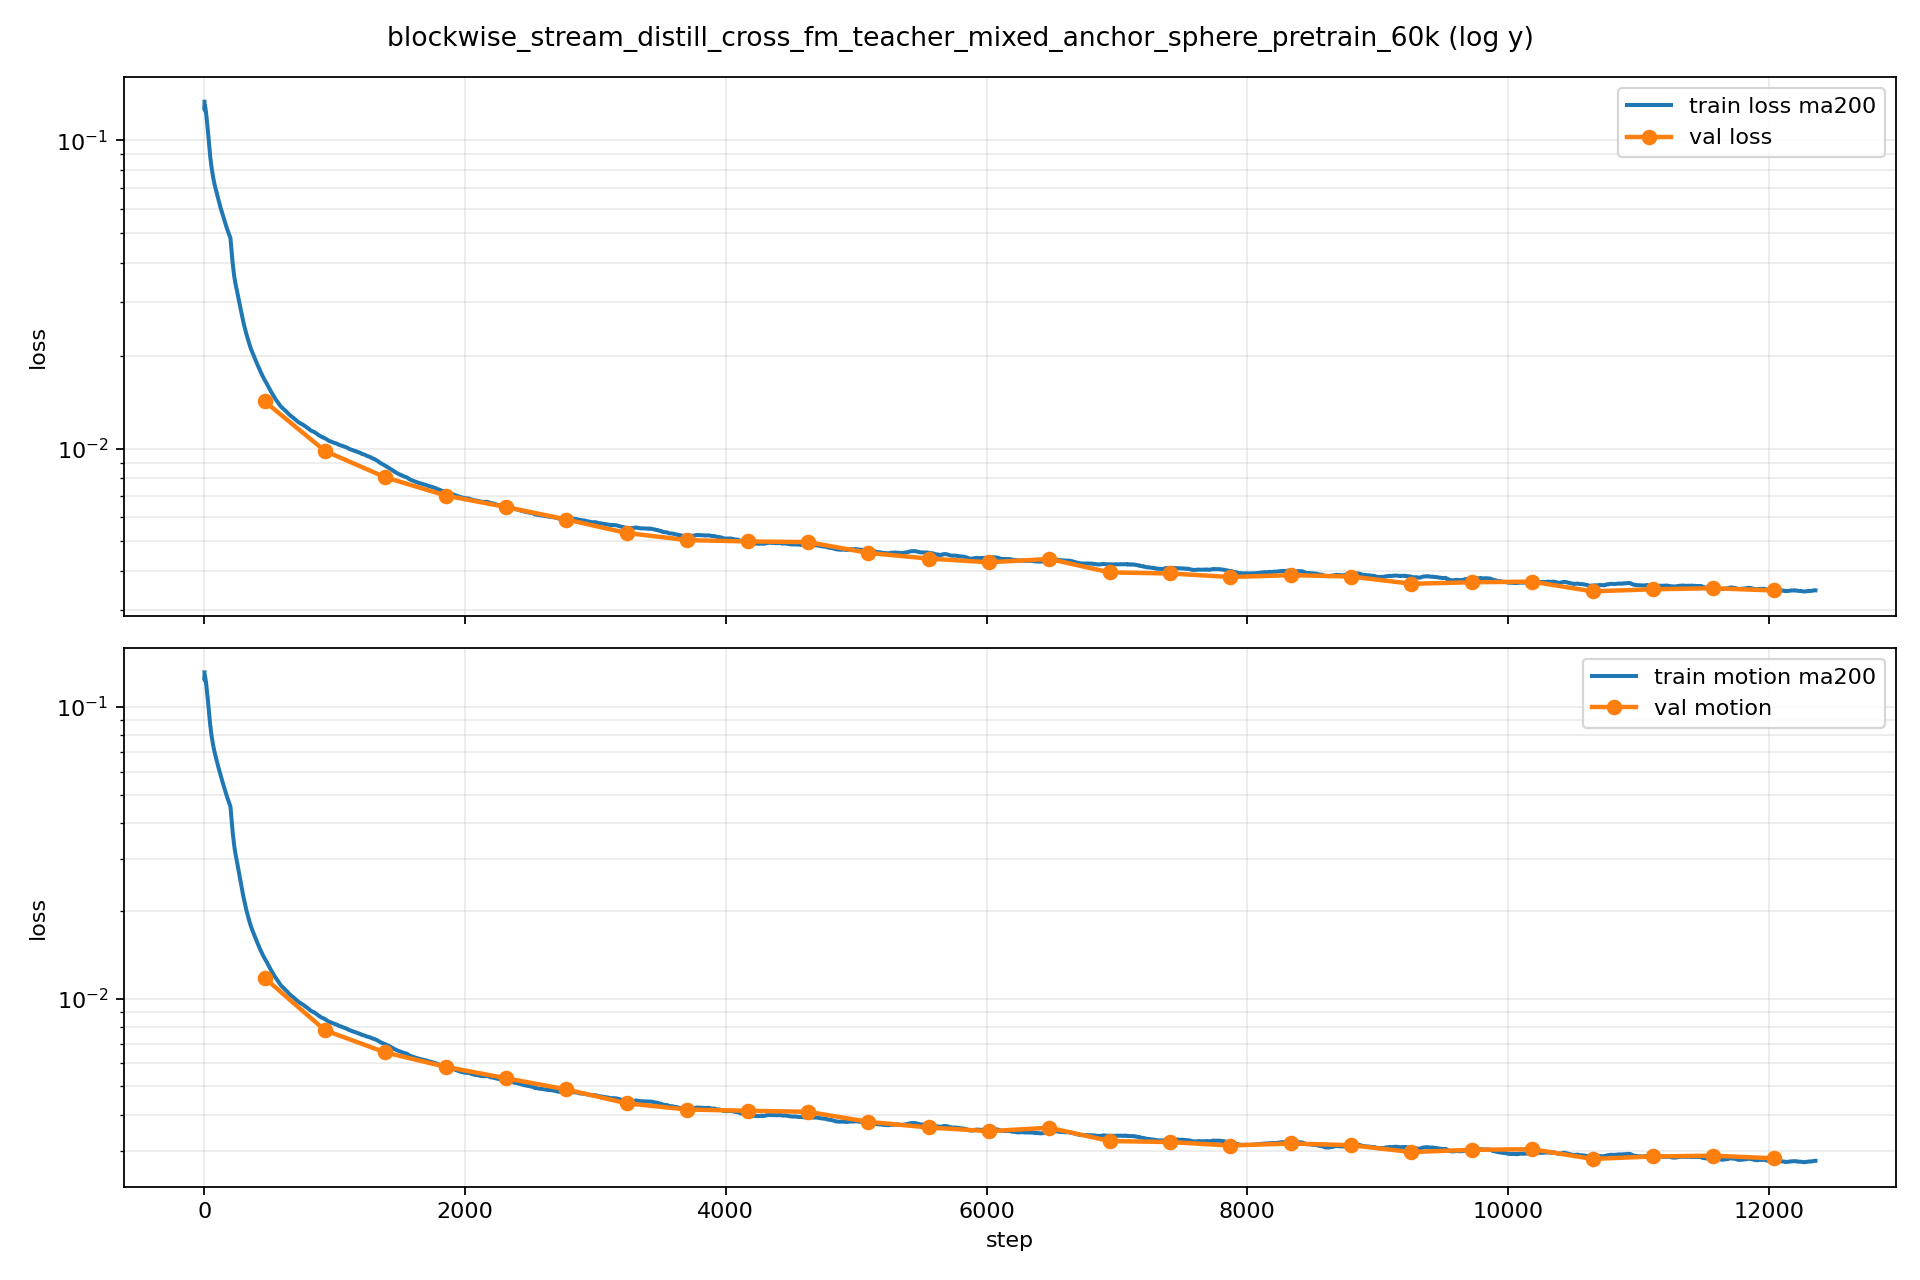
\includegraphics[width=\linewidth]{figures/loss_mixed_anchor_log.png}
  {\small Mixed-anchor student}
\end{minipage}
\caption{Training curves. Both variants converge smoothly. Real-anchor training is the safer default, while mixed anchors act as regularization rather than a consistently better objective.}
\label{fig:loss}
\end{figure}

\begin{figure}[t]
\centering
\begin{minipage}{0.48\textwidth}
  \centering
  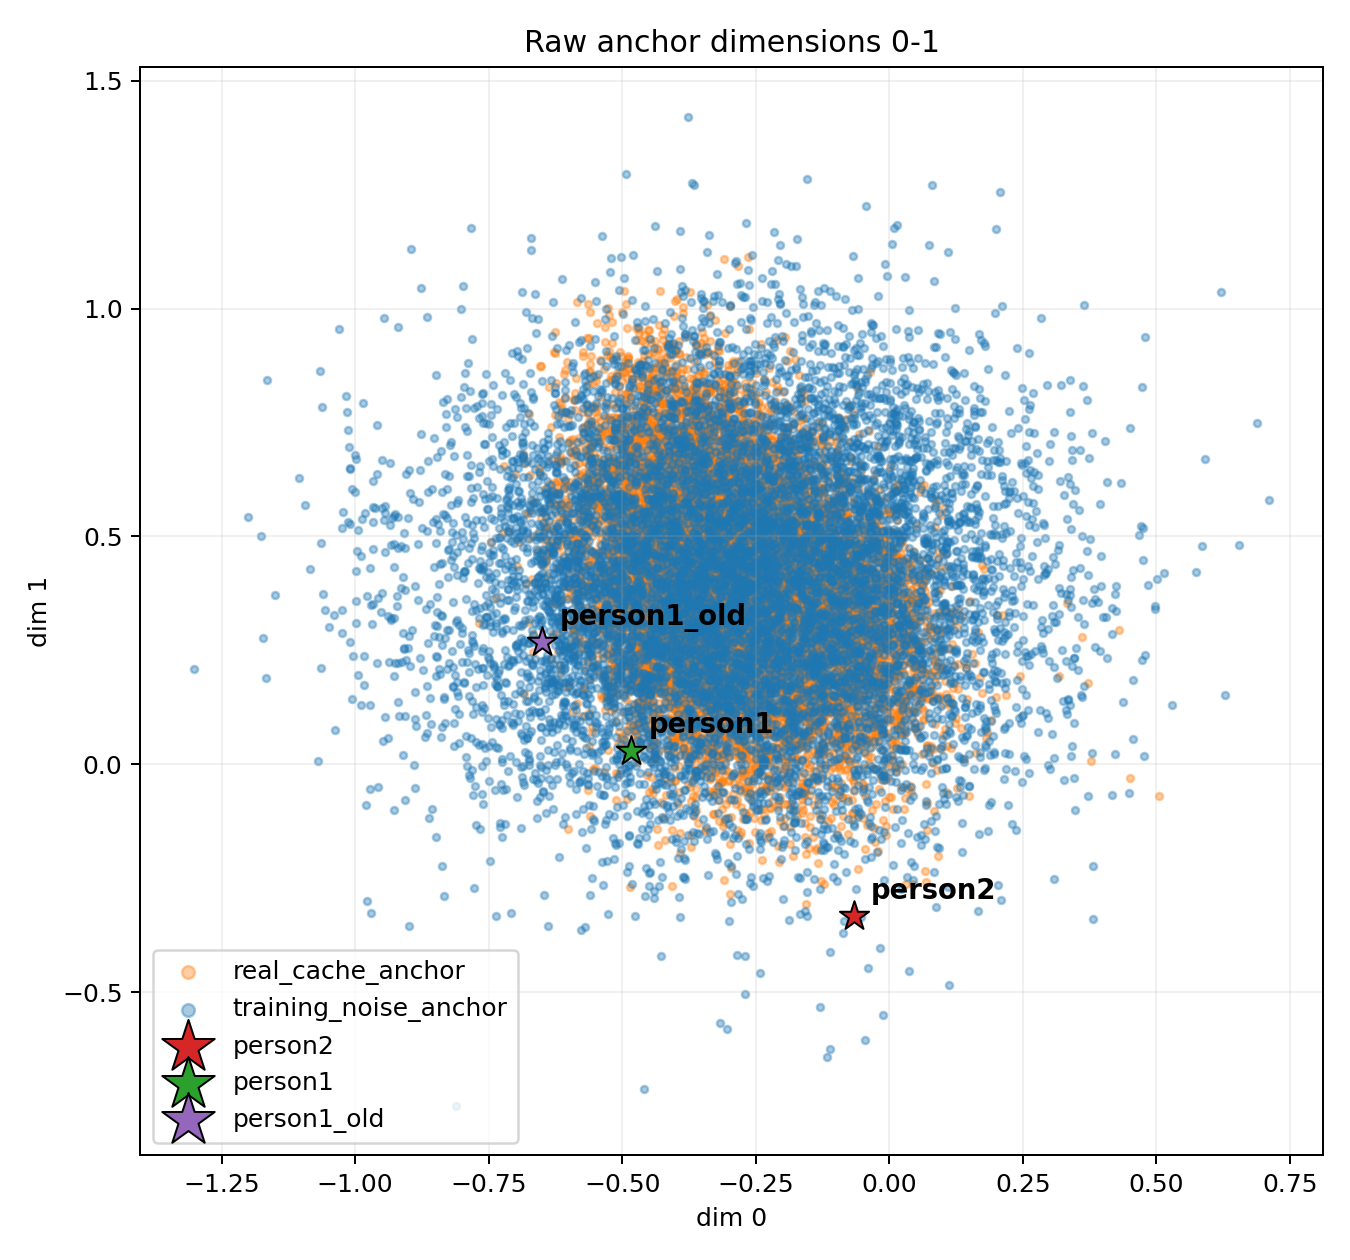
\includegraphics[width=\linewidth]{figures/anchor_raw_dims_0_1_person2.png}
  {\small Raw anchor dimensions 0--1}
\end{minipage}
\hfill
\begin{minipage}{0.48\textwidth}
  \centering
  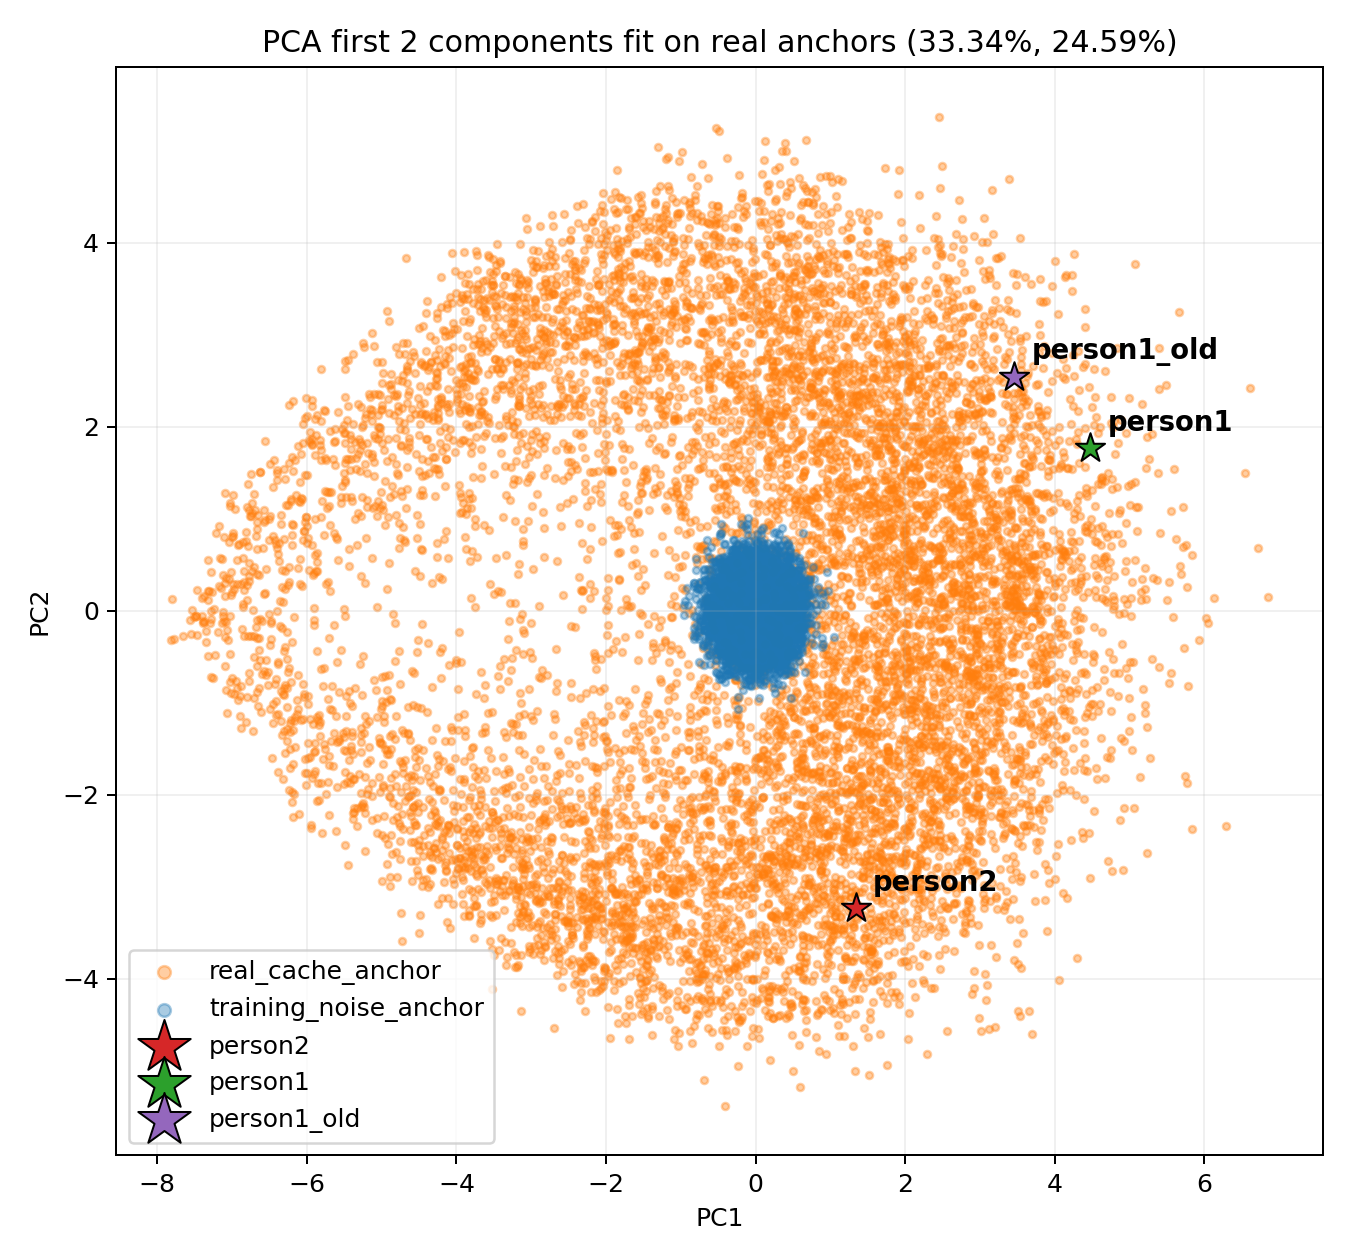
\includegraphics[width=\linewidth]{figures/anchor_pca2_person2.png}
  {\small PCA fit on real anchors}
\end{minipage}
\caption{Two views of anchor augmentation. In the raw coordinate slice, the synthetic sphere anchors broadly cover the selected reference anchors. In the real-anchor PCA view, however, the same samples concentrate near the center of the dominant real-anchor directions. The sphere therefore acts as a useful condition-space augmentation, but it is not a faithful replacement for the real anchor manifold.}
\label{fig:anchor_pca}
\end{figure}

The anchor study produced a nuanced result. In the original coordinate dimensions, synthetic sphere anchors can appear to cover the target references, so they are a reasonable form of anchor-space data augmentation. However, when PCA is fit on the real-anchor distribution, the synthetic sphere anchors are concentrated around the center of the first principal components. In 512 dimensions, large-radius random directions do not necessarily align with the low-dimensional real motion/identity manifold. This is why mixed noise anchors should be reported as an ablation and regularizer, not as the final default training strategy.

\begin{figure}[t]
\centering
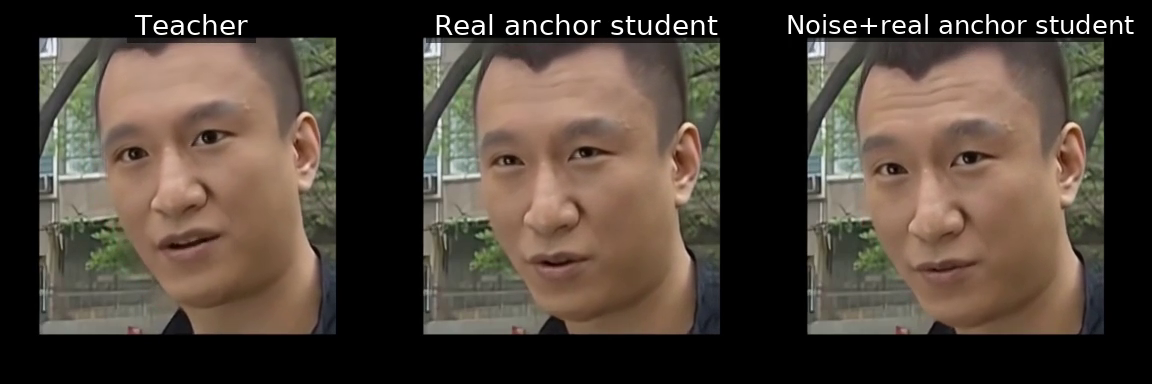
\includegraphics[width=\textwidth]{figures/comparison_teacher_real_noise_person2_t5.png}
\caption{Qualitative comparison frame from the 60-second Person2 three-way video: teacher, real-anchor student, and noise+real-anchor student. In this example, the mixed-anchor student produces a more conservative head pose than the teacher and preserves facial details such as forehead wrinkles more clearly, although this advantage is not consistent across all metrics. The full rendered sequence is used to check long-horizon identity consistency, and a 3-second preview is shown on the project page.}
\label{fig:qualitative}
\end{figure}

\subsection{Speed and Streaming Behavior}

The optimized teacher pipeline is close to the real-time boundary on a B20Z/B200-class GPU, especially after warm-up and with batched rendering, but it should not be interpreted as an order-of-magnitude faster-than-real-time system. The larger acceleration comes from AROD, which replaces the expensive teacher motion rollout with direct blockwise one-step denoising. In a fresh verification run with `verify\_blockwise\_distill.py' on a 60.03-second `person1 + test\_audio\_60s.wav' case, the teacher motion rollout took 29.38 seconds while AROD took 3.75 seconds, giving a 7.83$\times$ motion-generation speedup. A separate motion-only benchmark on the same case measured 26.01 seconds for the teacher and 3.25 seconds for AROD, or 8.00$\times$. Earlier verification of the same configuration recorded 10.24$\times$, so we describe the result as approximately 8$\times$ in the latest fresh run and capable of reaching about 10$\times$ under the same setup, rather than a fixed deterministic 10$\times$ for every run.

A real streaming demo also needs warm-up, rolling audio context, rolling motion history, frame buffering, stable playback, and a low-latency browser transport. Our current implementation should therefore be read as an offline Gradio demo plus a streaming-capable model design: the AROD student predicts short future blocks autoregressively, so it can be extended to rolling audio windows without changing the core motion model.

The largest remaining gap is interaction latency. Even when throughput is near real time, live streaming latency is bounded by audio chunk duration, backend processing time, render time, and playback buffering. Our current system is best described as \textit{real-time-capable} or \textit{streaming-capable}, not a fully optimized live streaming or video-call application.

%======================================================================
\section{Discussion}
%======================================================================

\paragraph{What worked.}
The strongest practical success is the decomposition. Keeping the DyStream renderer and teacher frozen makes the task tractable. Optimizing the runtime gives a fast demo. Distilling motion blocks gives a clear speed-quality trade-off. The blockwise denoising student also avoids the worst failure of plain regression: long-horizon identity collapse and severe slow-motion behavior.

\paragraph{What did not fully work.}
Pure cached-real supervised training from LRS3 motion latents can learn stable motion but may miss behaviors such as natural blinking. This suggests that teacher-generated motion contains useful priors beyond per-frame encoded ground truth. Synthetic anchor training also did not reliably improve objective metrics. It can regularize identity, but simple high-dimensional Gaussian or sphere noise does not match the real-anchor manifold.

\paragraph{Why not simply use one-step teacher FM?}
The original teacher can run with one denoising step, but the AR GPT component remains a bottleneck. Our student attacks that bottleneck by replacing sequential AR+FM rollout with direct blockwise motion prediction. This is why the student can be faster even when the teacher FM itself is already cheap.

\paragraph{Current best recommendation.}
For the final demo and report, the real-anchor student should be treated as the primary student model. The mixed-anchor model should be included as an ablation because it reveals a useful phenomenon: anchor perturbation can affect long-term identity consistency and mouth-motion strength, but naive noise does not consistently improve lip-sync metrics.

%======================================================================
\section{Limitations and Future Work}
%======================================================================

The current evaluation uses a small number of reference images and audio files. A more reliable conclusion needs a multi-speaker benchmark with averaged SyncNet, landmark, identity, and temporal metrics. The current web app is an offline generation demo. A true live streaming version would need lower-latency audio transport, rolling server-side scheduling, stronger front-end frame scheduling, and better handling of browser microphone noise.

Model-wise, the next step is to replace naive synthetic anchors with distribution-aware anchors. A promising direction is PCA/covariance sampling:
\begin{equation}
    \mathbf{r}_{\text{syn}} =
    \bar{\mathbf{r}} +
    U_k \Sigma_k^{1/2} \epsilon,
\end{equation}
where $U_k$ and $\Sigma_k$ come from real cached anchors. This would sample along the real anchor manifold instead of random 512D directions. Another direction is hybrid teacher/cache training: teacher targets preserve natural motion priors such as blinking, while cached-real targets improve grounding to actual LRS3 data.

%======================================================================
\section{Conclusion}
%======================================================================

StreamAvatar demonstrates a DyStream-based optimization and distillation path for real-time-capable audio-driven portrait animation. We successfully deployed and accelerated the teacher, built an offline AROD demo, trained blockwise motion students, and analyzed anchor conditioning. The results show that high-quality pretrained talking-head models can be pushed toward streaming-capable use without training a full renderer, but also that distilling autoregressive flow-matching behavior is not a trivial regression problem. Real anchors are currently the safest training condition; mixed noise anchors are useful as an ablation and regularizer but not a clear improvement. The project therefore provides both a working offline demo path and a set of lessons for future real-time avatar research.

\bibliographystyle{unsrt}
\bibliography{ref}

\end{document}
